\section{Lippukunnanjohtajan tervehdys}

\begin{multicols}{2}
\noindent Haara-, räystäs- ja tervapääskyt ovat jo aikaa sitten saapuneet, 
merihanhilla on jo poikasia ja kuuluipa pellon laidalta tuttu harmaasiepon 
''tsri tsri tsri''. Kevät on jo täällä ja kesä on aivan kulman takana. 
Valkovuokko, rentukka ja kirsikka ovat täydessä kukassa, mutta vielä on 
ensimmäisen satakielen laulu kuulematta. Onneksi kesällä järjestetään 
lippukunnan \textit{Satakieli}"-kesäleiri! Leirin lisäksi kesällä 
järjestetään \textit{Variksen vavahdus} "=vaellus ja 
\textit{Piisaminhäntä}"-melonta.

Alkuvuoteen on jälleen mahtunut monenlaista partiotekemistä kuten 
laskiaisriehaa, minihaikkia, partioparaatia ja lippukuntaretkeä. Olen 
haltioissani siitä, kuinka paljon erilaista toimintaa pieni lippukuntamme on 
pystynyt järjestämään; kevään toimintamme on kartuttanut käyntikertoja 
yli kuusisataa! Tämä ei ole mikään itsestäänselvyys, vaan mielekäs 
toiminta vaatii aina vapaaehtoisia, tekijöitä ja johtajia -- unohtamatta itse 
osallistujia, joita ilman tekeminen menettää merkityksensä.  

Osin partiotoiminnan mahdollistaa se, että lippukuntamme on rekisteröity 
yhdistys. Sillä on vuosikokouksen valitsema hallitus, joka vastaa 
toimintasuunnitelman toteutumisesta, päättää kalusto- ja muista 
hankinnoista, ylläpitää jäsenrekisteriä, anoo avustuksia, edustaa 
lippukuntaa piirin aluetapaamisissa\ldots\ Lippukunnan hallinto on yleistäen 
kuin valtion, kunnan tai jonkin yrityksen hallinto pienoiskoossa, joten 
partiotoiminnan tähän välillä tylsältäkin vaikuttavaan osaan tutustuminen 
tarjoaa johtajalle paljon hyödyllisiä tietoja ja taitoja. Haluaisitko sinä 
tutustua lippukunnan hallituksen tehtäviin? 

Kevättä varjosti Kurkisuon Rusakoiden perustajajäsenen ja ensimmäisen 
lippukunnanjohtajan, Eddien poisnukkuminen. ''Yritä jättää tämä maailma 
vähän parempana kuin sen löysit,'' kehotti Baden"-Powell viimeisessä 
viestissään partiolaisille. Sama ilmaisu löytyy SP:n partioneuvoston 
hyväksymistä partion yhteiskunnallisen toiminnan linjauksista. Nykyisenä 
lippukunnanjohtajana olen vahvasti sitä mieltä, että Eddie otti kehotuksesta 
vaarin.

Partioterveisin ja Eddien muistoa kunnioittaen

\noindent\null\hfill Janne

% \smallskip

\begin{center}
	\noindent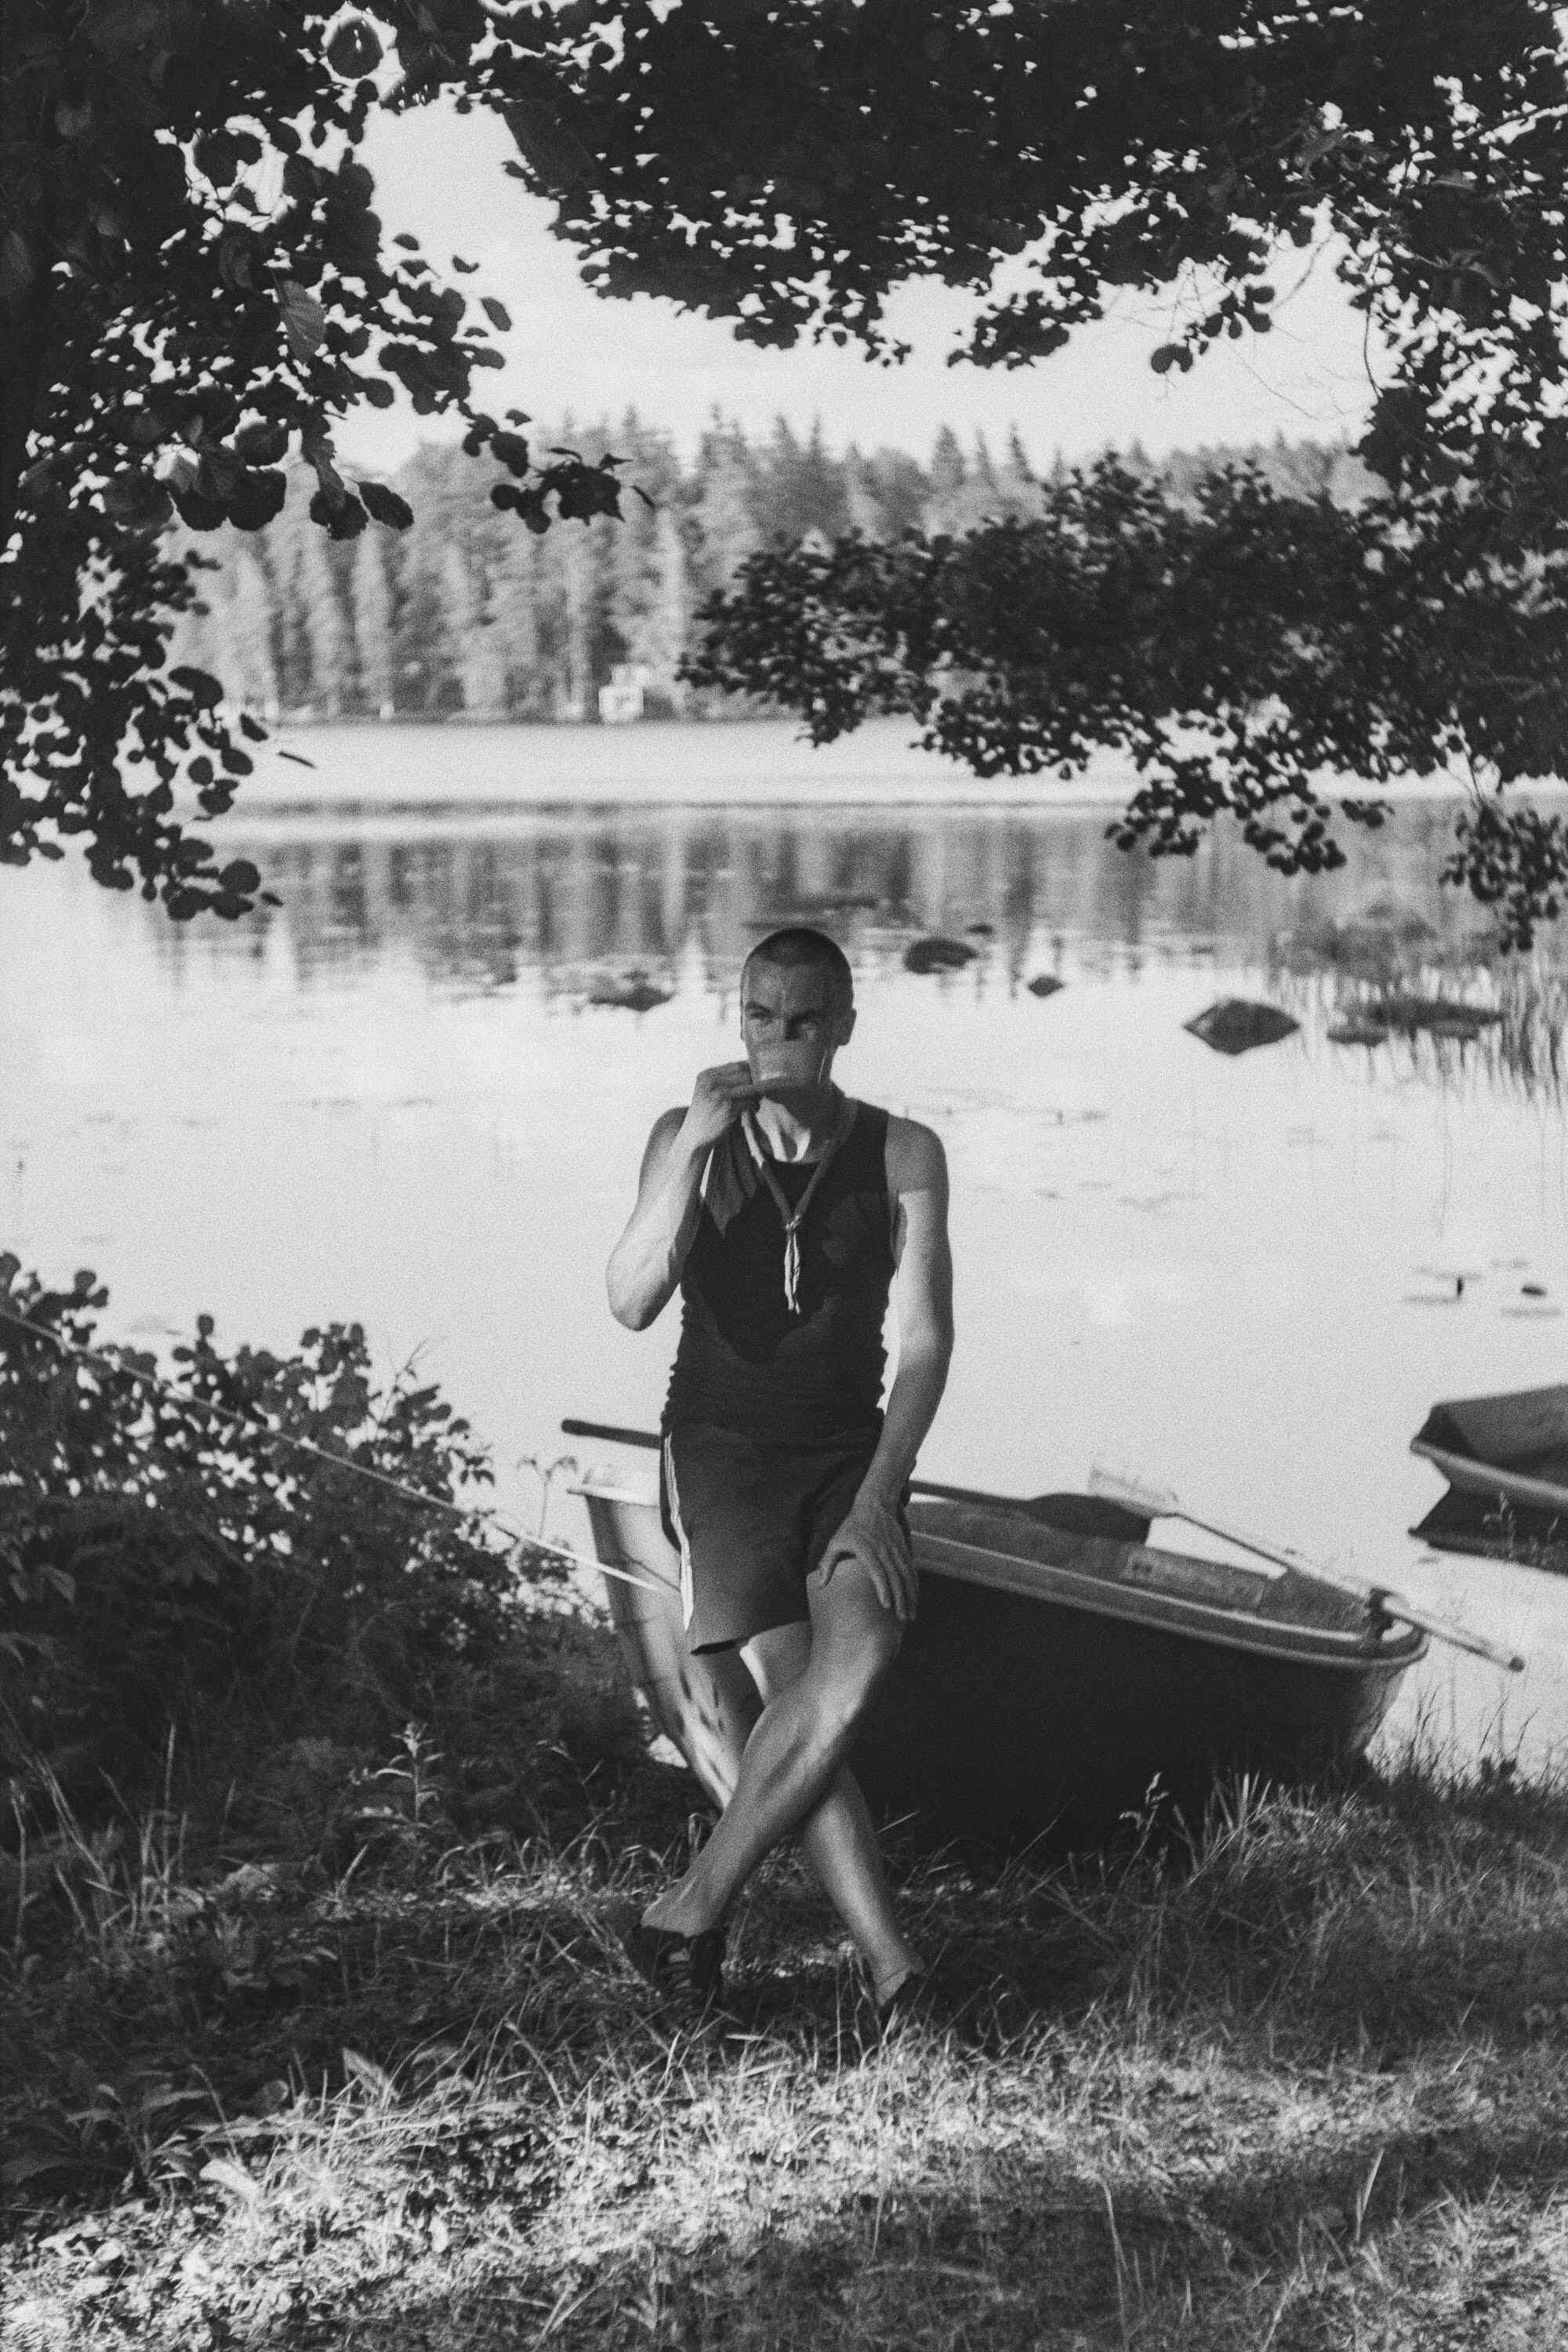
\includegraphics[width=0.85\linewidth,,trim={0cm 3.5cm 0cm 10.5cm},clip]{assets/lpkjohtajantervehdys}
\end{center}

% \smallskip

\noindent\null\hfill Kuva: Tanguy

\vspace*{-1.5cm}

\end{multicols}
